
\section{Report (2016-02-01)}

I want to focus on sense classification, mostly due to the fact that this is provided as a separate task with provided training and test data. If there is time left, I could implement this module into the previous year's best performing end-to-end discourse parser. After having studied the previous year's systems, I have come to the conclusion that there is a gap in representation learning approaches. While I probably will not be alone in this decision (just look at last year's EMNLP), I might be able to contribute with some non-obvious ideas.

There were only two systems that used semantic representations, both from University of Dublin, and both performing relatively weakly in the task. The other submissions are only using ''shallow'' features. \cite{okita_dcu_2015} focuses on using paragraph vectors along with some additional features to improve sense classification. They obtain reasonable F-score for explicit senses (.88), while the implicit sense classification is quite bad (.11). The implicit sense classification is mainly bad due to low recall (.15), while the precision is on par with explicit sense classification. Furthermore, they find that the classification task struggles with classes with explicit connectives where the surface form is occurring in more than one class. The second paper by \cite{wang_dcu_2015} is not focusing on sense classification and thus not provide much detail about its results there. Overall, its results are somewhat disappointing.

Beyond last year's submissions, \cite{ji_representation_2014} has implemented a parser using representation learning for the RST treebank which uses another discourse framework compared with PDTB. This one shows significant improvements compared to previous SOTA on the treebanks, but the results are in no way comparable with the PDTB. Still, it is the first paper (that I could find) that uses representation learning in a discourse parsing context, and it does so successfully which makes me want to at least look into their manually selected features later on. I am honestly somewhat surprised that none of the other systems looked into using this for the task, especially since the authors of the overview papers considered its results interesting enough to briefly mention it.

What I am most excited about is the idea of applying findings from architectures for the Stanford Natural Language Inference Corpus \citep{bowman_large_2015}. This is a classification task that I consider to be fairly similar to the sense classification task, and there are several interesting model implementations with strong results I want to further explore. Their website\footnote{\url{http://nlp.stanford.edu/projects/snli/}} especially mentions \cite{mou_recognizing_2015} as a particularly efficient recursive neural network model with strong results. \cite{cheng_long_2016} is a LSTM network model, albeit not as efficient, but receives the highest score so far. Unfortunately, neither of these seem to have published their code which would mean some reimplementation efforts. I don't mind since I would like to learn TensorFlow anyway, and Google's Mat Kelcey has already some code I could work off of, albeit the performance is not as good\footnote{\url{https://github.com/matpalm/snli_nn_tf}}.

That said, there are some things to keep in mind. First of all, neural network approaches are mainly known to be good when there are a lot of training data. That is not necessarily the case here. If the approaches above fail, I will look into if it is possible to use other, more sparse data friendly, architectures with the semantic representations. Also, \cite{braud_comparing_2015} compared shallow features with some dense vector representations and found that shallow features still receive SOTA for implicit discourse relation identification. They do not seem to base any of their findings on word2vec vectors though, which is the kind of features that is allowed in the closed shared task. Also, their concatenation methods differ from the kind of architectures I have in mind. I will have to read this paper more carefully, and see what kind of dead ends I might be able to avoid.

\emph{Last minute update}: I just found out about \cite{zhang_shallow_2015} from EMNLP 2015 which is a shallow convolutional neural network which reaches SOTA on implicit discourse recognition (which is not entirely the same task) on PDTB, making some of the previous worries about neural network approaches less worrisome. I am going to get a good understanding of their approach, read up on the NLI papers, and see how I can combine their efforts.

But first things first: I need to set up a baseline. Here are some suggestions:

\begin{itemize}
	\item Try to break out the sense classifier from previous year's best performing paper \citep{wang_refined_2015}. They use two separate classifiers for explicit and non-explicit senses, based on the original architecture in \cite{lin_pdtbstyled_2014}, while adding a few extra features to boost the performance. The code is freely available, so it should be doable. Although it is unclear if this is actually the best model for sense classification.
	\item Do the same thing, but for the original architecture. \citep{lin_pdtbstyled_2014}. The code base is also available.
	\item Try to figure out which of the systems perform best on
	\item Implement some other simple system, e.g. an SVM bag-of-words model, potentially with brown clusters due to them
\end{itemize}

I'm leaning towards the having both the first suggestion, using \cite{wang_refined_2015}, as well as the SVM. The first suggestion due to me wanting to potentially incorporate my classifier into their system, and SVM for its usage as baseline in \cite{zhang_shallow_2015} that I just found.

\subsection{Questions!}

\begin{itemize}
	\item Is this a good plan?
	\item Is using \cite{wang_refined_2015} as a baseline a good idea?
	\item Am I fooling myself by believing that I can learn anything from studying NLI architectures?
	\item The sense classes are rather imbalanced (see Table \ref{tbl:sense_frequency}). Do you know of any general methods on how to deal with this?
	\item What am I missing?
\end{itemize}

\section{Report (2016-02-25)}

Since last time, I have been focusing on three things:

\begin{itemize}
	\item Learning theory behind neural networks, convolutional NN, recurrent NN, and recursive NN.
	\item Learning tensorflow
	\item Setting up experimental architecture.
\end{itemize}

The first point has been going well. I have a sort of reasonable understanding of the maths behind it (backprop is still magic). I have a good understanding of the theory behind the Tree-Based Convolutional Neural Network (TB-CNN) as described in \cite{mou_recognizing_2015}. I found this particular model interesting due to its incorporation of tree structures into a (for neural networks) easily trainable CNN architecture while receiving very strong results on the NLI task. I haven't looked quite as closely to the other candidates yet.

For the rest to make sense, I will have to make a short summary of how TB-CNN differs from common CNN architectures. Basically, they have incorporated a tree-structure into the convolutional operation. While a common CNN in NLP applications (such as \cite{kim_convolutional_2014}) runs its convolution on \emph{sequentially} adjacent word features, TB-CNN runs its convolution on \emph{hierarchically} adjacent word features according to its dependency tree. Moreover, while a common CNN has one weight matrix per feature map which is used across all words, TB-CNN has one weight-matrix per \emph{dependency label}.

After going through the NN theory, I started to go deep into Tensorflow which has been fairly straight-forward. This is when I started to realize that implementing TB-CNN will be more difficult than I first imagined, due to the unorthodox convolutional operations in the model which aren't easily supported by neither Tensorflow nor Theano (which are the two frameworks I feel comfortable working with). I still haven't completely given up on being able to implement it, I find its incorporation of tree structures in CNN very interesting and intuitive, but currently I think my time is better spent implementing simpler models.

I have the following models in mind for this:

\begin{itemize}
	\item A simple logistic regression model just as a proof of concept that my architecture works. This is almost done (see below).
	\item An SVM to have my baseline somewhat ready. This should be quick.
	\item Incorporating a feed-forward NN model that has been implemented and released for the NLI corpus, with reasonable results. This should be quick.
	\item A very successful NN model for sentiment analysis is the Recursive Neural Network by \cite{socher2013recursive}. This, similarly to the TB-CNN incorporates tree structures into its semantic composition, while actually having a Theano implementation for me to work from.
	\item \cite{cheng_long_2016} is an LSTM model that currently has the best score for the NLI corpus. Despite having the best score and seeming quite implementable, due to the long training times for these types of model I am somewhat doubtful that I would like to work with them. It is still worth considering, though.
	\item And just for completion, \cite{kim_convolutional_2014} is a simple CNN model for sentence processing. This is attractive due to being relatively efficient to train.
\end{itemize}

To put this work into some context, I will describe my experimental architecture that I have implemented this last week.

\subsection{Experimental architecture}

In the planning and subsequent implementation of the architecture, I focused on having a very modular design, making it easy to plug in and try out new models, features, and different training data. For this to work, each module need to be agnostic about what the others do, and simply expect to receive and output data according to a standardized API. This resulted in the following modules:

\subsubsection{extractors} Implements a number of feature extraction models. It takes sentences as input and transforms them into e.g. word2vec features, brown clusters, etc. Outputs a feature matrix (words x word\_features).

\subsubsection{resources} Takes care of training/test/dev data by reading data and massaging it into adhering to a standardized API. It outputs a feature tensor (sentences x words x word\_features) given a set of extractors.

\subsubsection{models} Takes a feature tensor as input, reshapes the tensor into its required shape, and trains a model on this. It thereafter saves the model, and tests it given dev or test data. This makes implementing new models fairly easy. Currently, a logistic regression model is at least trainable.

\subsubsection{test\_report} Saves results along with its configuration and training model in a transparent way. This isn't built yet, but I need some sort of structure to make sense of the hundreds of different configuration permutations I'm going to have. The experimental framework Sacred\footnote{\url{http://sacred.readthedocs.org/en/latest/}} seem to promise to do just this in an automated fashion, and I will probably try to incorporate it into my architecture.

At the time of writing, everything is implemented except for testing the trained model, and test\_report.py. I hope to finish this in a few days and thereafter focus on implementing models. All sorts of parameters and hyperparameters are collected in one big config file.


\subsection{Things to ponder}

One big difference between the NLI task and this task is the number of output classes (see table \ref{tbl:sense-hierarchy}). While NLI has 2 different classes, PDTB has 16. Furthermore, some instances have \emph{two} concurrent classes, that is, an instance can have e.g. \emph{CONTINGENCY} and \emph{Temporal.Synchrony} at the same time. If we were to treat all of these as atomic units, we would have 56 unique classes to predict. Most of these dual-class instances are very rare and I am thinking about ignoring these for now. Furthermore, I am also thinking about focusing on getting the top-level hierarchy right for now, that is, only classifying \emph{TEMPORAL}, \emph{CONTINGENCY}, \emph{COMPARISON}, and \emph{EXPANSION}, and look into the second level hierarchy when I have a working model for the first hierachy. I think splitting up the classification into two separate hierarchies to be beneficial for accuracy as well.

I am still uncertain how I can make use of the implicit/explicit relations. Obviously explicit gives me an extra feature which helps a lot, but I am uncertain if it is best to have an entirely separate classifier for implicit relations, or treat them as the explicit relations with a specific IMPLICIT feature in place of its explicit connective.

Another thing I wonder is: can I have access to a GPU to run my experiments on? It would be nice to be able to speed up the tuning a bit.

I think that's it for now!

\section{Report (2016-03-22)}

This will only be a quick description of my two current models with some initial results.

Word vectors below refers to either randomized fixed-sized vectors, or pre-trained word2vec.

Each instance has the following arguments:

\begin{itemize}
	\item connective\_token: Refers to the binding tokens between the two arguments. This can be null if instance is of type Implicit (underlined).
	\item arg2\_text: Refers to the text string which is syntactically binded with connective\_token (bolded).
	\item arg1\_text: Refers to the other argument (cursive).
\end{itemize}


\begin{exe}
\ex \emph{Boeing would make cost-of-living adjustments projected to be 5 for each year of the contract} \underline{though} \textbf{the union has called the offer insulting}.\label{exemple:boeing}
\end{exe}


\subsection{SVM Baseline}

The SVM is a simple model, doing the following:
\begin{enumerate}
	\item Generate word vectors for all words for the training instance's arguments.
	\item Calculate the mean word vector (centroid) for each argument.
	\item Concatenate the arguments' centroid vectors.
	\item Train the SVM classifier on this feature vector.
\end{enumerate}


I'm using the default parameters as set by scikit-learn. This include a non-linear kernel, RBF:

\begin{verbatim}
	SVC(C=1.0, cache_size=200, class_weight=None, coef0=0.0,
    decision_function_shape=None, degree=3, gamma='auto', kernel='rbf',
    max_iter=-1, probability=False, random_state=None, shrinking=True,
    tol=0.001, verbose=False)
\end{verbatim}

\subsection{CNN Model}

The CNN model is based on the tutorial \emph{Implementing a CNN for Text Classification in TensorFlow}\footnote{\url{http://www.wildml.com/2015/12/implementing-a-cnn-for-text-classification-in-tensorflow/}}. This implements a model very similar to \cite{kim_convolutional_2014}, which is a text classification model using convolutional neural networks with word vectors for sentence-level classiciation tasks. It learns task-specific vectors by tuning the word vectors during training, and at the time gave SOTA results for a number of sentiment analysis tasks. See \ref{fig:cnnarchitecture}.

\begin{figure}[h]
	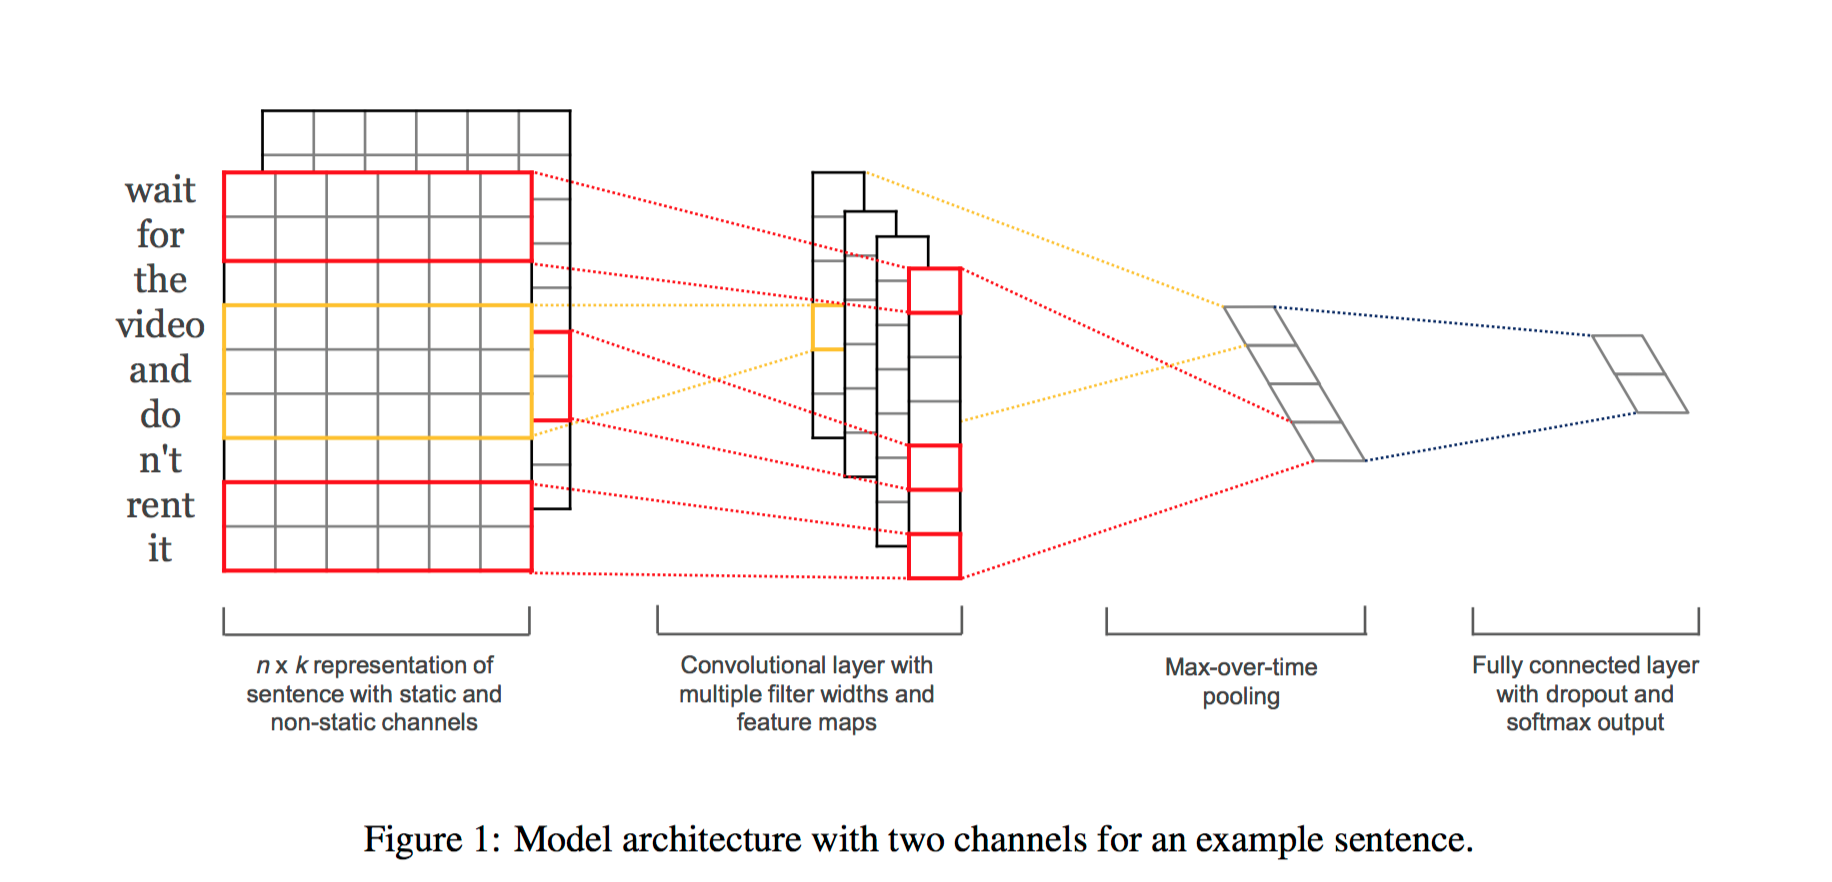
\includegraphics[width=0.9\textwidth]{images/cnn_architecture}
	\label{fig:cnnarchitecture}
\end{figure}

The model requires a fixed number of words for training per argument. Each argument, as listed above, therefore has a \emph{max\_words} setting, which is currently set to 5 for connective tokens and 25 for each argument text. If the argument is shorter than the max setting, we pad the sentence with additional words. If it's longer, we cut the sentence at the given point. Each arguments instance matrix are concatenated, making the input matrix dimensionality (25+25+5, embedding\_dimensionality).

This too has a number of tunable features that I have yet to look closer into. The two most prominent are the number of convolutional filters, as well as the filter sizes. A filter size determines the span of the convolutional operation, e.g, a filter size of 2 looks at bigrams. Each filter is randomly initialized, and will through training tune into finding different features in the sentences. I also plan on experimenting with different number of convolutional layers with different pooling algorithms.

\begin{verbatim}
	embedding_dim: 300
	filter_sizes: [1,2]
	num_filters: 128
	dropout_keep_prob: 0.5
	l2_reg_lambda: 3
	batch_size: 128
	num_epochs: 100
	evaluate_every: 100
	checkpoint_every: 100
	allow_soft_placement: true
	log_device_placement: false
	max_words_in_sentence: 25
\end{verbatim}

\subsection{Results so far}

So far, the SVM is doing better, although CN seems to be somewhat better at classifying implicit relations. The reason for this is that when the connective is not present, it defaults to the class EntRel which is neither explicit nor implicit, while the CNN behaves more randomly. I haven't looked into what kind of results randomly assigned labels would give, so I'm not sure it actually beats random yet.

I'm going to read up on other CNN models to get some tips on how I can best structure the input (perhaps split up each argument input into separate convolutional networks which are then merged. I think I saw someone doing something like this, but I have had trouble finding it.). Somewhat surprisingly, randomized vectors actually performs \emph{better} than word2vec. If this has to do with randomized vectors being more easily tuned, or if there is a bug somewhere, I'm not sure. I will have to look into this further.

\subsection{Todo}

Whether or not I will send something into the shared task is depended on whether I can make this model work. I won't have time for a lot of tuning, so I will try to read as much as possible on different convolutional neural network implementations to get a good overview of what parameters seem to work and what I should think of.
